\documentclass[conference]{IEEEtran}
\usepackage{graphicx}

% correct bad hyphenation here
\hyphenation{op-tical net-works semi-conduc-tor}


\begin{document}
%
% paper title
% can use linebreaks \\ within to get better formatting as desired
\title{Suboptimal Time Management Technique for Non-ideal Shared space}


% author names and affiliations
% use a multiple column layout for up to three different
% affiliations
\author{\IEEEauthorblockN{Praveen Kumar Pendyala}
\IEEEauthorblockA{Information and Communication Engineering\\
Technische Universitat Darmstadt\\
Email: m@praveen.xyz}}

% make the title area
\maketitle


\begin{abstract}
%\boldmath
Time management is an asset and a liability. Lack of proper time management may put oneself on a depression feedback loop [1]. Time management is a melange of various aspects - scheduling tasks, execution and time line corrections, to name a few. Each of these aspects can be thought as a subproblem in our attempts to tackle the grand problem - Optimal Time Management. In addition to these subproblems, we must accept the fact that we live in a non-ideal world along with many others - shared space.  The paper presents a pseudo adaptive, suboptimal Time Management technique taking other players - shared space and non-ideal world, into consideration.
\end{abstract}


% For peer review papers, you can put extra information on the cover
% page as needed:
% \ifCLASSOPTIONpeerreview
% \begin{center} \bfseries EDICS Category: 3-BBND \end{center}
% \fi
%
% For peerreview papers, this IEEEtran command inserts a page break and
% creates the second title. It will be ignored for other modes.
\IEEEpeerreviewmaketitle


\section{Introduction}
% \IEEEPARstart
Time and Time Management are of paramount importance. This brings in an obvious urge to develop various techniques for an optimal time management technique. Starting from marking calender to a rigid time plan accounting for each hour of a day. There are a whole lot of techniques to make a basic plan, some of which will be covered in the existing literature section. One major aspect of time management is making a perfect schedule but an even more crucial part kicks in during its execution. There are several factors that could keep one from meeting their time plan. Stress, Bad planning, Lack of self control etc., which are mostly internal factors - in the sense that their correction is solely dependent on the individual. There are also external factors that could affect ones time plan - factors which the individual may not have anticipated or predicted at the time of planning.

The source of all the factors that affect time plans, broadly speaking, are a result of the fact that we live in a shared space where we are affected not only by our own actions but also by the choices of those around us and that we live in a non-ideal world where most events are probability based, not guided by any standard Uncertainty Principle, brings in more players into the equation. All these complex parameters would push any purely mathematical or conceptual approach to derive an optimal time plan into solving an NP-Hard problem [2]. One has to live with a suboptimal time plan for a given situation, iterate it based on their needs and arrive at an acceptable compromise between an ideal and executable plan.

The following contents of the paper are divided into four sections. Section II. Existing literature would focus on some of the existing techniques for Time management. Followed by Section III. Execution and Evaluation which is completely spanned by a case study where the subject employs an adaptive time management technique for their day to day activity for a fortnight. We will then conclude with Section IV. Conclusions, where would be highlighting the key aspects of our argument and how we derived or observed them in the case of the test subject.

\section{Existing literature}
There is plethora of research related to Time Management (TM) techniques and surveys depicting the outcomes of adopting or otherwise of a TM technique. [3], [4] and [5] centered their work around the impact of TM in an academic context, backing their claims through surveys with varying size of sample space and interpretations but similar outcomes. Time Management behaviors may have beneficial effects on tensions and job satisfaction but not on job performance. Contrary to popular claims, time management training was not found to be effective [6]. This controverts the hypothesis and findings of [7] and [8].

The common shortcoming in all these literatures is their failure to account that test subjects could be influenced by a plethora of external and internal factors. All these influencing factors, broadly speaking, are a result of Non-idealistic behavior and shortcomings of the test subjects and negative, intended or unintended, influence from peers, colleagues and other indirect players on test subject's attempts in keeping up with their schedule. Attempts have been made to evaluate the extent of influence by a common factor, tendency of procrastination, on the effective execution of ones time plan [9], [10]. 

The common shortcoming in all these literatures is their failure to account that test subjects could be influenced by a plethora of external and internal factors. All these influencing factors, broadly speaking, are a result of Non-idealistic behavior and shortcomings of the test subjects and negative, intended or unintended, influence from peers, colleagues and other indirect players on test subject's attempts in keeping up with their schedule. Attempts have been made to evaluate the extent of influence by a common factor, tendency of procrastination, on the effective execution of ones time plan [9], [10]. 

The common shortcoming in all these literatures is their failure to account that test subjects could be influenced by a plethora of external and internal factors. All these influencing factors, broadly speaking, are a result of Non-idealistic behavior and shortcomings of the test subjects and negative, intended or unintended, influence from peers, colleagues and other indirect players on test subject's attempts in keeping up with their schedule. Attempts have been made to evaluate the extent of influence by a common factor, tendency of procrastination, on the effective execution of ones time plan [9], [10]. 

\section{Execution and Evaluation}
We analyzed the day-to-day life executions of a test subject and how they divulge from their expected time plan. A qualitative note on the external factors causing the time-line diversion is also provided corresponding to each diversion.

\begin{figure}[hb]
  \centering
  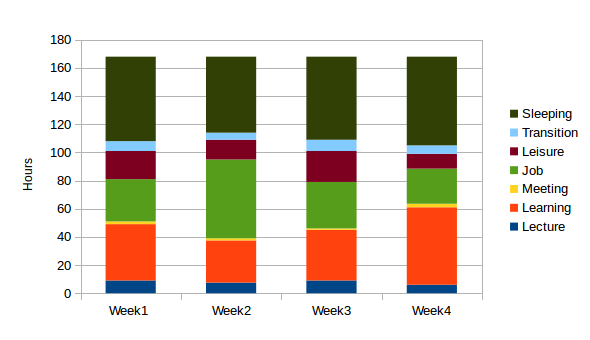
\includegraphics[width=3.7in]{bar}
  \caption[]
   {Close up Hemidactylus sp., which is
   part the genus of the gecko family. It is the
   second most speciose genus in the family.}
\end{figure}

\begin{figure}[hb]
  \centering
  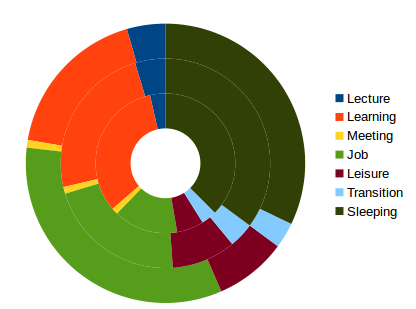
\includegraphics[width=3.7in]{donut}
  \caption[]
   {Close up Hemidactylus sp., which is
   part the genus of the gecko family. It is the
   second most speciose genus in the family.}
\end{figure}

% use section* for acknowledgement
\section*{Acknowledgment}
The author would like to extend his gratitude to the Telecooperation Group of TU Darmstadt for providing the required tools and resources, which form the basis for Test Subject Data collection and served as starting for this paper.



% trigger a \newpage just before the given reference
% number - used to balance the columns on the last page
% adjust value as needed - may need to be readjusted if
% the document is modified later
%\IEEEtriggeratref{8}
% The "triggered" command can be changed if desired:
%\IEEEtriggercmd{\enlargethispage{-5in}}

% references section

\begin{thebibliography}{1}

\bibitem{IEEEhowto:}
\emph{Yoga Journal}, \relax May-Jun 1976, pp. 17.

\bibitem{IEEEhowto:}
Aaronson, Scott. \emph{"NP-complete problems and physical reality."} ACM Sigact News 36.1, 2005, pp. 30-52.

\bibitem{IEEEhowto:}
Britton, Bruce K., and Abraham Tesser. \emph{"Effects of time-management practices on college grades."} Journal of educational psychology 83.3 (1991): 405.

\bibitem{IEEEhowto:}
Macan, Therese H., et al. \emph{"College students' time management: Correlations with academic performance and stress."} Journal of educational psychology 82.4 (1990): 760.

\bibitem{IEEEhowto:}
Misra, Ranjita, and Michelle McKean. \emph{"COLLEGE STUDENTS'ACADEMIC STRESS AND ITS RELATION TO THEIR ANXIETY, TIME MANAGEMENT, AND LEISURE SATISFACTION."} American Journal of Health Studies 16.1 (2000): 41-51.

\bibitem{IEEEhowto:}
Macan, Therese Hoff. \emph{"Time management: Test of a process model."} Journal of applied psychology 79.3 (1994): 381.

\bibitem{IEEEhowto:}
Adams, Gary A., and Steve M. Jex. \emph{"Relationships between time management, control, work–family conflict, and strain."} Journal of Occupational Health Psychology 4.1 (1999): 72.

\bibitem{IEEEhowto:}
Waterworth, Susan. \emph{"Time management strategies in nursing practice."} Journal of Advanced Nursing 43.5 (2003): 432-440.

\bibitem{IEEEhowto:}
Lay, Clarry H., and Henri C. Schouwenburg. \emph{"Trait procrastination, time management, and academic behavior."} Journal of Social Behavior and Personality (1993).

\bibitem{IEEEhowto:}
Gafni, Ruti, and Nitza Geri. \emph{"Time management: Procrastination tendency in individual and collaborative tasks."} Interdisciplinary Journal of Information, Knowledge, and Management 5 (2010): 115-125.



\end{thebibliography}




% that's all folks
\end{document}


